\documentclass[aspectratio=169]{beamer}
%
% Choose how your presentation looks.
%
% For more themes, color themes and font themes, see:
% http://deic.uab.es/~iblanes/beamer_gallery/index_by_theme.html
%
\mode<presentation>
{
  \usetheme{metropolis}      % or try Darmstadt, Madrid, Warsaw, ...
  \usecolortheme{metropolis-imagelab} % or try albatross, beaver, crane, ...
  \usefonttheme{structurebold}  % or try serif, structurebold, ...
  \setbeamercolor{background canvas}{bg=white}
  \setbeamertemplate{navigation symbols}{}
  \setbeamertemplate{bibliography item}{\insertbiblabel}
  %\setbeamertemplate{caption}[numbered]
} 
\usepackage[english]{babel}
\usepackage[utf8x]{inputenc}
\usepackage{listings}             % Include the listings-package
\hypersetup{
    colorlinks = true,
    linkcolor = {black},
    urlcolor = {mImagelabRed}
}

\DeclareMathOperator*{\argmin}{arg\,min}

\title[Support Vector Machines]{Support Vector Machines}
\subtitle{Pattern Recognition and Machine Learning - MuMeT 2017}
\institute{University of Modena and Reggio Emilia}
\author{Davide Abati}
\date{June 23th, 2017}

\def\thisframelogos{}

\newcommand{\framelogo}[1]{\def\thisframelogos{#1}}

\begin{document}

\framelogo{logo_unimore_white.png}

\bgroup
\renewcommand{\insertframenumber}{}
\begin{frame}[noframenumbering]
  \titlepage
\end{frame}
\egroup

\begin{frame}{Support Vector Machines (SVM)}
Very famous supervised learning algorithm:
\begin{itemize}
\item performs \textbf{binary} classification (can be adapted for multiclass problems)
\item is \textbf{linear} (in its original formulation) 
\item main feature: chooses the decision boundary that \underline{maximizes the margin} between positive and negative examples
\end{itemize}
\begin{columns}
\begin{column}{0.5\textwidth}
\begin{center}
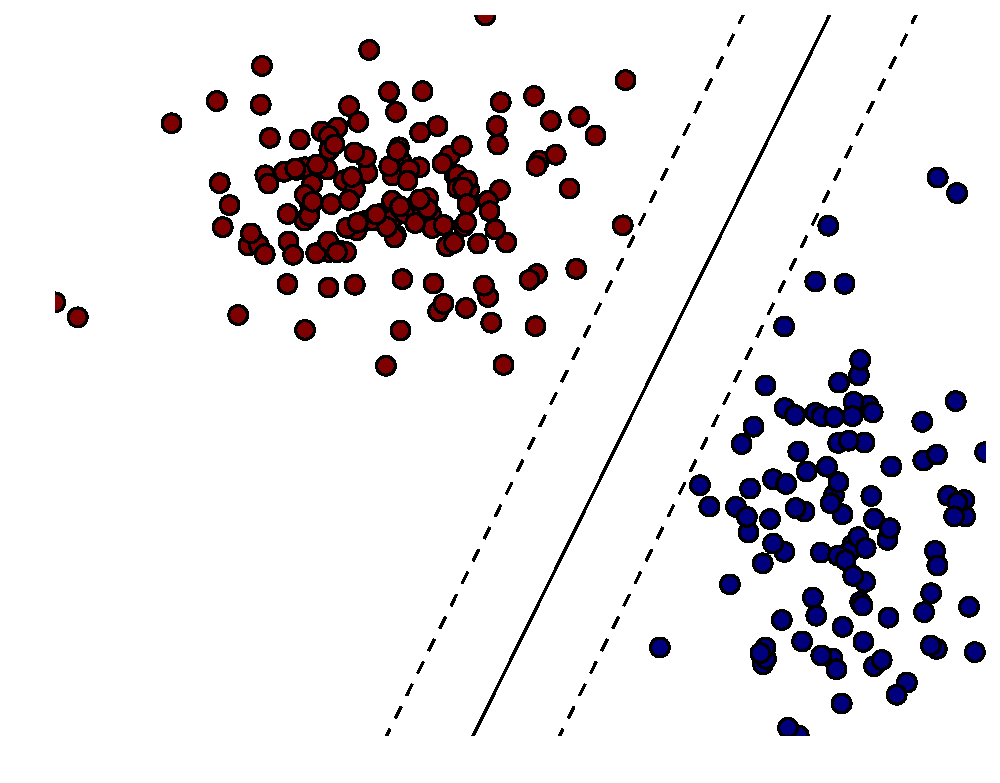
\includegraphics[width=0.7\textwidth]{img/svm/max_margin.pdf}
\end{center}
\end{column}
\begin{column}{0.5\textwidth}
How do you find such line?
\end{column}
\end{columns}
\end{frame}
\begin{frame}{SVM: problem setting}
\begin{itemize}
\item we have a set of examples $\{\vec{x_i}\}_{i=1}^N$, with label $\{y_i\}_{i=1}^N$
\begin{itemize}
\item $\vec{x_i}$ is a feature vector
\item $y_i \in \{-1, 1\} \quad \forall i=1,\ldots,N$
\end{itemize}
\item the line that maximizes the margin (hyperplane) is identified by
\begin{itemize}
\item the vector $\vec{w}$ orthogonal to it
\item the intercept $b$
\end{itemize}
\end{itemize}
\end{frame}
\begin{frame}{SVM: hard margin optimization}
It can be shown that solving this constrained optimization problem maximizes the margin:
\begin{equation*}
\begin{aligned}
& \min_{\vec{w},b} & & \frac{1}{2}||w||^2\\
& \text{s.t.} & &  y_i(\vec{w}^T\cdot\vec{x_i} + b)>1 & \forall i=1,\ldots,N
\end{aligned}
\end{equation*}
After estimating $\vec{w}$ and $b$, the decision rule for an unknown example $\vec{u}$ is simply:
\begin{equation*}
f(\vec{u}) = \text{sign}(\vec{w}^T\cdot\vec{u} + b)
\end{equation*}


\end{frame}
\begin{frame}{SVM: non separable data}
What if you cannot find a linear decision boundary?
\begin{center}
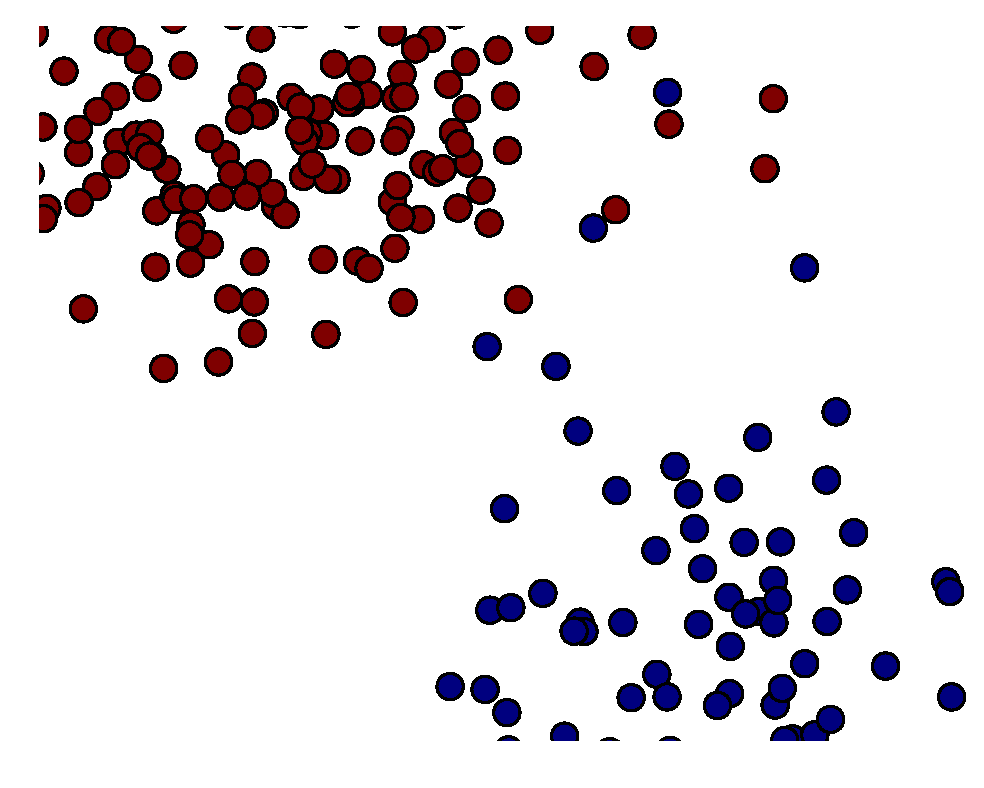
\includegraphics[width=0.35\textwidth]{img/svm/non_linear_data.pdf}
\end{center}
Two solutions:
\begin{itemize}
\item introduce slack variables $\xi_i$ (patch solution)
\item kernel trick
\end{itemize}
\end{frame}
\begin{frame}{SVM: soft margin optimization}
Introduce a slack variable $\xi_i$ for every training example
\begin{equation*}
\begin{aligned}
& \min_{\vec{w},b} & & \frac{1}{2}||w||^2 + C\sum_{i=1}^N\xi_i\\
&\text{s.t.} & & y_i(\vec{w}^T\cdot\vec{x_i} + b)>1-\xi_i & \forall i=1,\ldots,N\\
& & & \xi_i > 0 & \forall i=1,\ldots,N
\end{aligned}
\end{equation*}
where $C$ is a tradeoff between the margin maximization and the slack variable minimization.

The decision rule for an unknown example $\vec{u}$ does not change:
\begin{equation*}
f(\vec{u}) = \text{sign}(\vec{w}^T\cdot\vec{u} + b)
\end{equation*}


\end{frame}
\newlength{\overwritelength}
\newlength{\minimumoverwritelength}
\setlength{\minimumoverwritelength}{1cm}
\newcommand{\overwrite}[3][mImagelabRed]{%
  \settowidth{\overwritelength}{$#3$}%
  \ifdim\overwritelength<\minimumoverwritelength%
    \setlength{\overwritelength}{\minimumoverwritelength}\fi%
  \stackrel
    {%
      \begin{minipage}{\overwritelength}%
        \color{#1}\centering\small #3\\%
        \rule{1pt}{9pt}%
      \end{minipage}}
    {\colorbox{#1!50}{\color{black}$\displaystyle#2$}}}

\begin{frame}{SVM: kernels}
Math guys find out that if you employ Lagrangian multipliers to solve the optimization the problem, you need to find the extrema of the following function ($\{\alpha\}_{i=1}^N$ are the lagrangian multipliers of each training example):
\begin{equation}
L = \sum_i \alpha_i - \frac{1}{2} \sum_i \sum_j \alpha_i \alpha_j y_i y_j \overwrite{\vec{x_i} \cdot \vec{x_j}}{!!!!!!}
\end{equation}
\end{frame}
\begin{frame}{SVM: kernels (2)}
You can replace that dot product with a kernel $\phi$
\begin{equation}
L = \sum_i \alpha_i - \frac{1}{2} \sum_i \sum_j \alpha_i \alpha_j y_i y_j \phi(\vec{x_i}, \vec{x_j})
\end{equation}
Choose a kernel:
\begin{itemize}
\item linear: $\phi(\vec{x_i}, \vec{x_j}) = \vec{x_i}\cdot\vec{x_j}$
\item polynomial: $\phi(\vec{x_i}, \vec{x_j}) = (\vec{x_i}\cdot\vec{x_j}+c)^d$
\item gaussian: $\phi(\vec{x_i}, \vec{x_j}) = \exp(-\frac{||\vec{x_i}-\vec{x_j}||^2}{2\sigma^2})$
\end{itemize}
This way, you draw the line in a transformed space, leading to non linear decision boundaries in the original space!
\end{frame}
\begin{frame}{SVM example}
Using a linear kernel:
\begin{figure}
\begin{tabular}{cc}
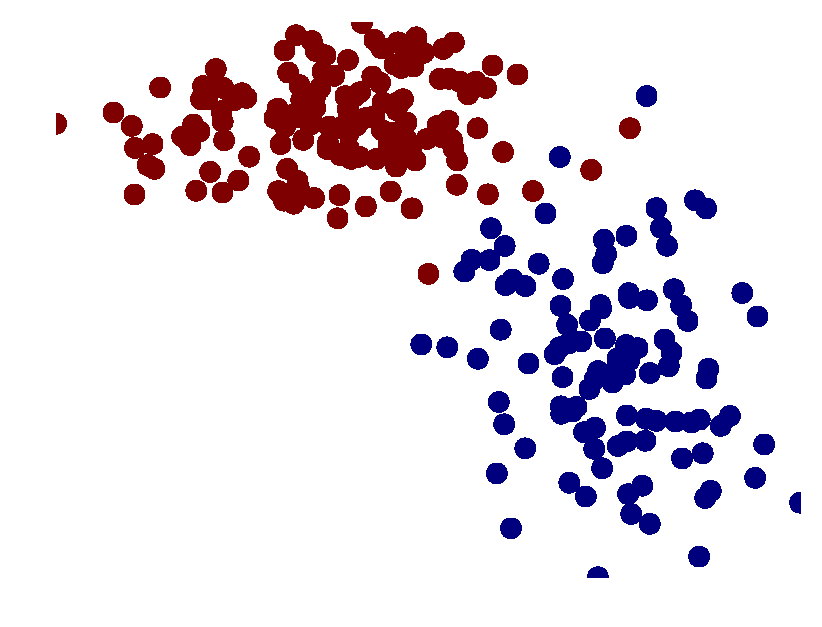
\includegraphics[width=0.4\textwidth]{img/svm/linear_kernel_11.pdf}&
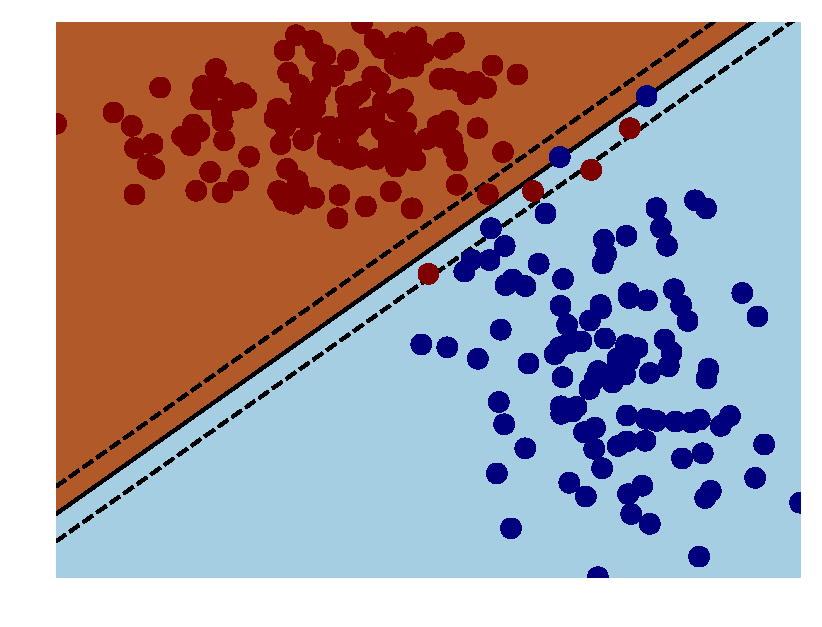
\includegraphics[width=0.4\textwidth]{img/svm/linear_kernel_12.pdf}
\end{tabular}
\end{figure}
\end{frame}
\begin{frame}{SVM example}
Using a rbf (gaussian) kernel:
\begin{figure}
\begin{tabular}{cc}
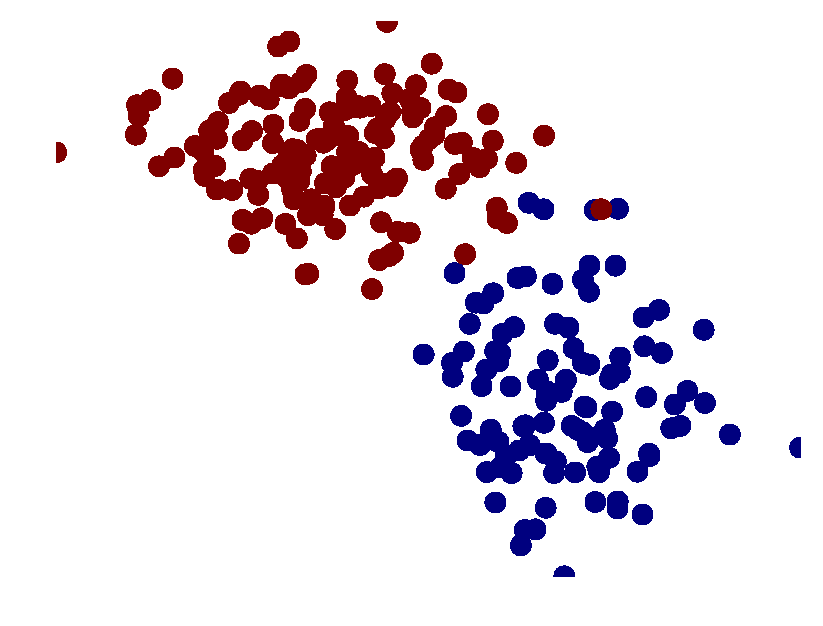
\includegraphics[width=0.4\textwidth]{img/svm/rbf_kernel_11.pdf}&
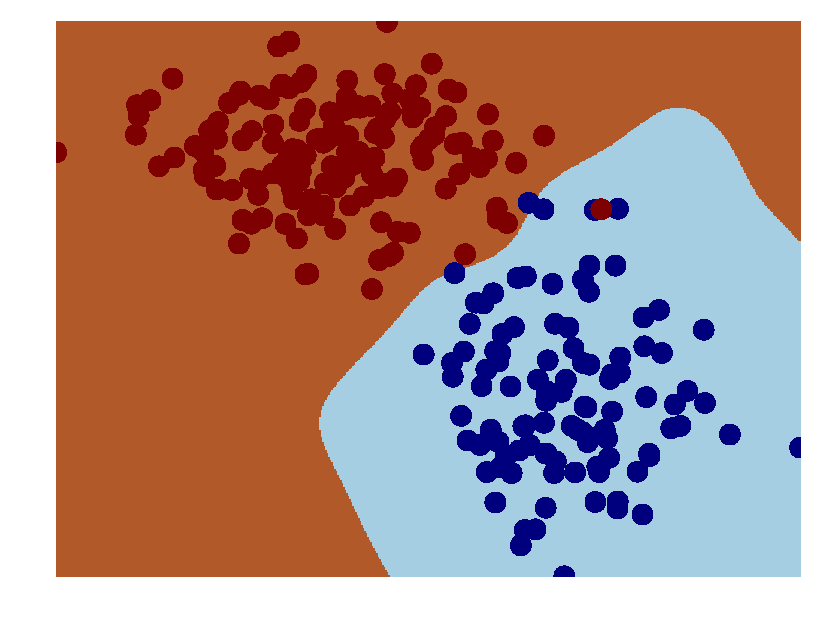
\includegraphics[width=0.4\textwidth]{img/svm/rbf_kernel_12.pdf}
\end{tabular}
\end{figure}
\end{frame}
\begin{frame}{SVM example (2)}
Using a linear kernel:
\begin{figure}
\begin{tabular}{cc}
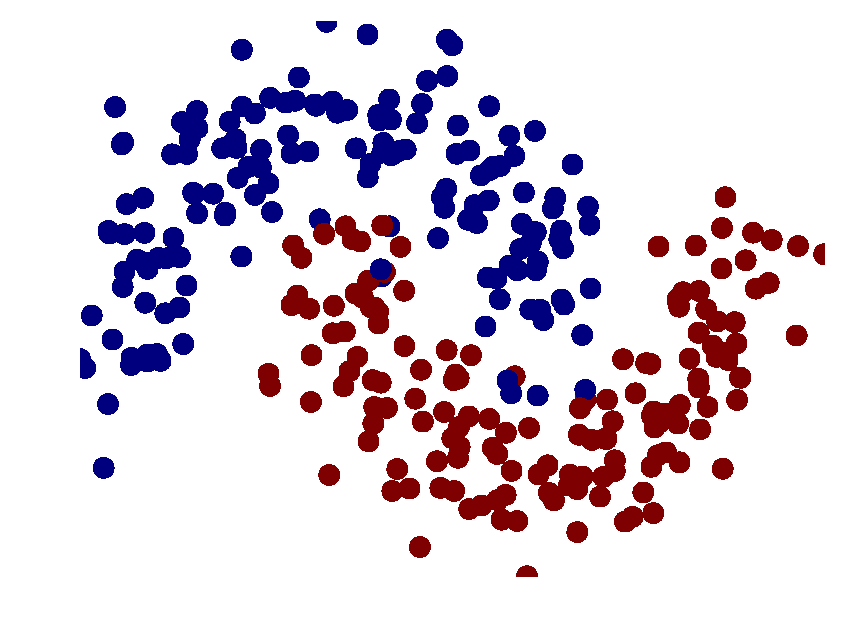
\includegraphics[width=0.4\textwidth]{img/svm/linear_kernel_21.pdf}&
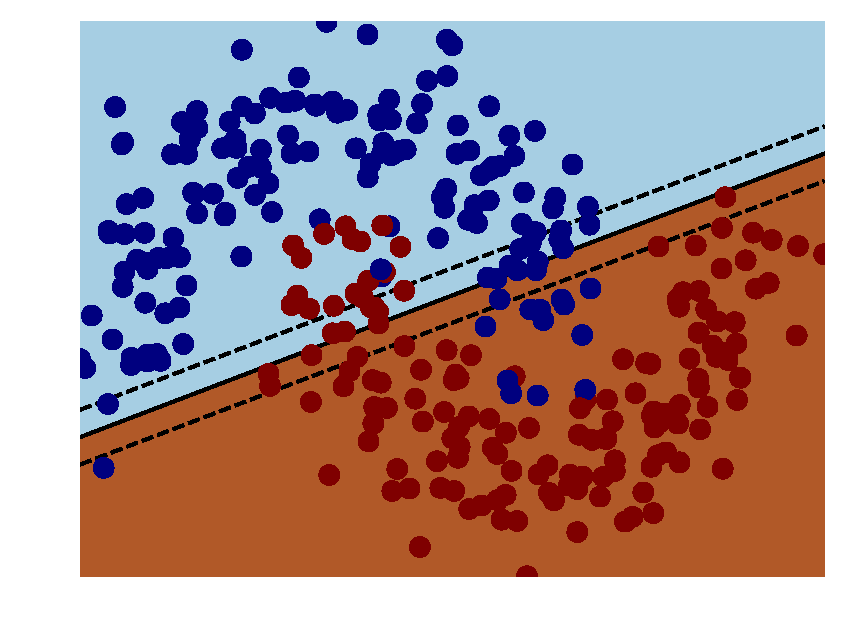
\includegraphics[width=0.4\textwidth]{img/svm/linear_kernel_22.pdf}
\end{tabular}
\end{figure}
\end{frame}
\begin{frame}{SVM example (2)}
Using a rbf (gaussian) kernel:
\begin{figure}
\begin{tabular}{cc}
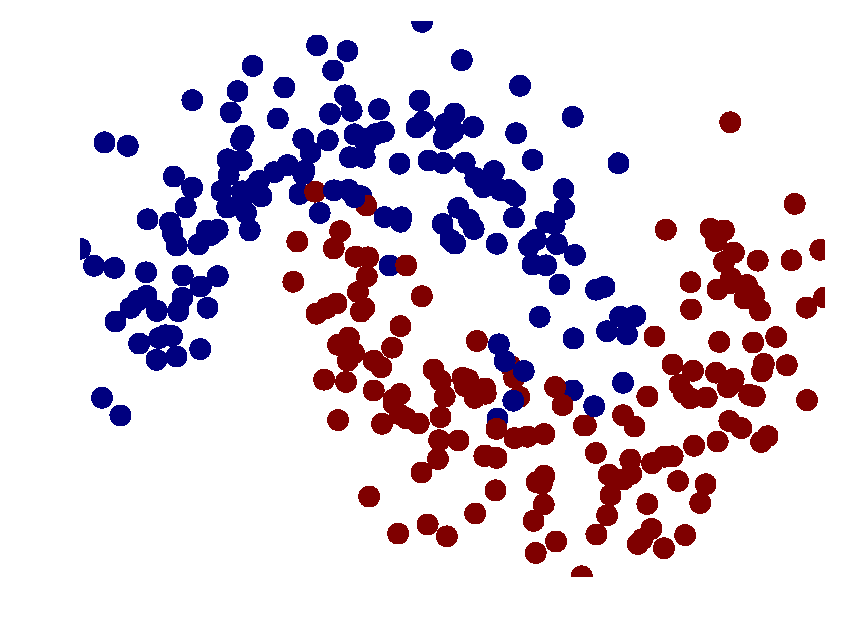
\includegraphics[width=0.4\textwidth]{img/svm/rbf_kernel_21.pdf}&
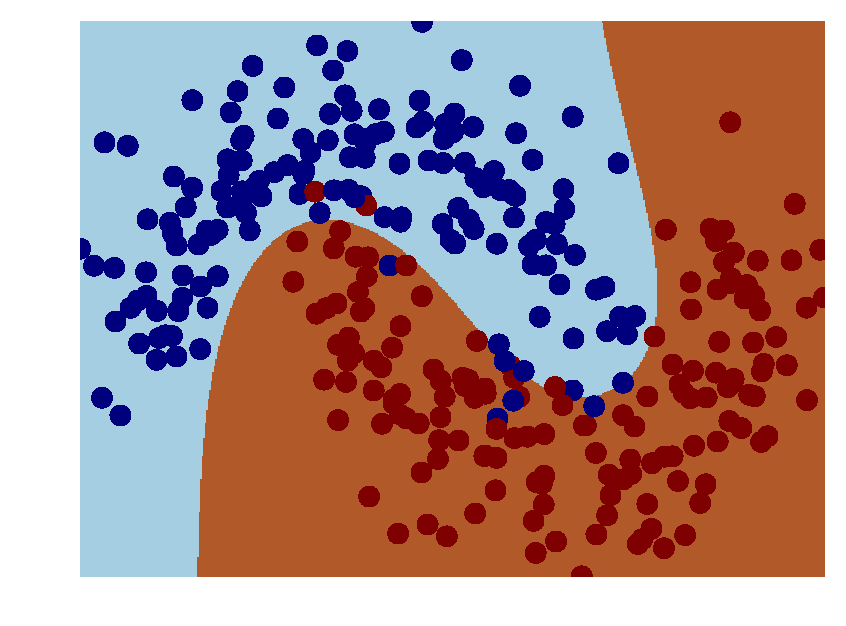
\includegraphics[width=0.4\textwidth]{img/svm/rbf_kernel_22.pdf}
\end{tabular}
\end{figure}
\end{frame}

\section{Application: people vs non people classification}
\begin{frame}{SVM for people detection}
We will discriminate between people and non people
\begin{figure}
\begin{tabular}{cc}
\small{people} & \small{non people}\\
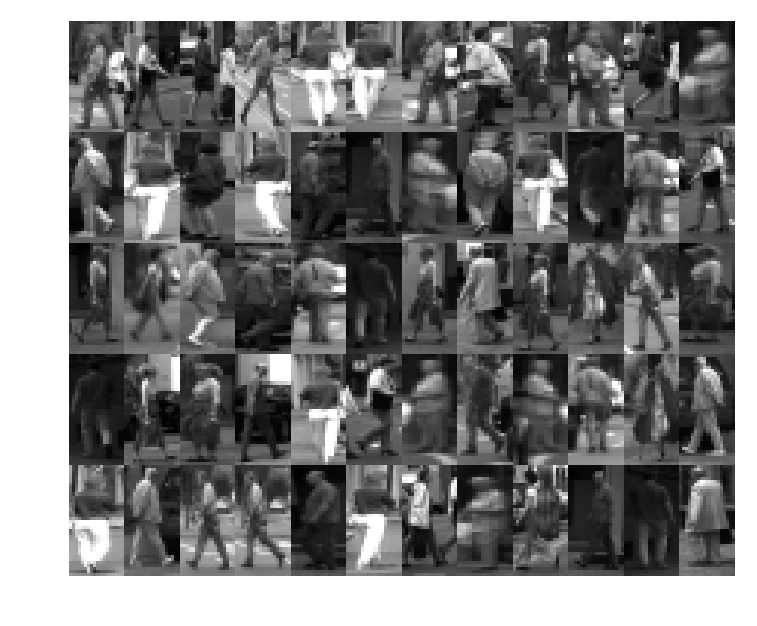
\includegraphics[width=0.4\textwidth]{img/people_classification/people.pdf}&
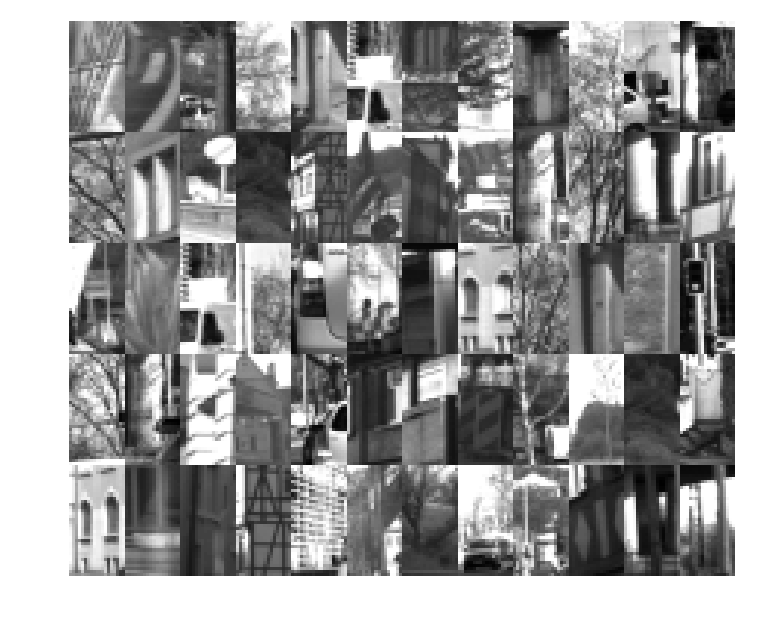
\includegraphics[width=0.4\textwidth]{img/people_classification/non_people.pdf}
\end{tabular}
\end{figure}
\end{frame}
\begin{frame}{SVM for people detection (2)}
Pipeline for people vs non people classification with \textbf{HOG features}:
\begin{itemize}
\item load training examples (images, HOG features, labels)
\item load test examples (images, HOG features, labels)
\item choose a kernel (linear or rbf) and a value for C and initialize a SVM model 
\begin{itemize}
\item use \href{http://scikit-learn.org/stable/modules/generated/sklearn.svm.SVC.html}{sklearn.svm.SVC}
\end{itemize}
\item fit a SVM model on training examples
\begin{itemize}
\item use \href{http://scikit-learn.org/stable/modules/generated/sklearn.svm.SVC.html\#sklearn.svm.SVC.fit}{SVC.fit()}
\end{itemize}
\item use model for computing predictions on test examples
\begin{itemize}
\item use \href{http://scikit-learn.org/stable/modules/generated/sklearn.svm.SVC.html\#sklearn.svm.SVC.predict}{SVC.predict()}
\end{itemize}
\end{itemize}
\end{frame}

\end{document}